\documentclass[a4paper]{article}
\usepackage[english]{babel}
\usepackage[utf8x]{inputenc}
\usepackage{amsmath}
\usepackage{graphicx}
\usepackage[colorinlistoftodos]{todonotes}

\title{Assignment 1: Search Algorithms Report}
\author{Stephen Weinpahl (sjw170) and Michael Trinh (mht46)}
\date{}

\begin{document}
\maketitle
\section*{{Preface}}

\textit
{The searching python file contains five complete searching algorithms to find a path from the start point to the end point in the maze. An initial problem file provides the maze number which relates to a file that describes the maze’s structure, the start and end points and the algorithm which is used to solve the maze. The included python file needs all related maze files to be included in the same directory that the python file is in. The files methods as well as their purpose are described in the readme. Several libraries were used to assist in the implementation of the algorithms and visualization, including the deque library from collections which implements a queue, the heapq library which implements a min heap and the matplotlib and numpy libraries which implement the maze and data visualization. This report will focus on comparing several well known algorithms performance on solving the maze and will look to explain their behavior. }
\newline
\newline
\section*{{Problem Description}}
\begin{itemize}
    \item States: Location of the agent on a grid.
    \item Initial State: The initial state is a point on the grid that the agent starts at.
    \item Goal State: Reaching a specific cell in the grid without colliding with any blocked cells.
    \item Actions: The agent can move left, right, up, or down, but cannot move diagonally.
    \item Transition Model: The result of moving to a cell.
    \item Action Cost: Moving left/right has an action cost of 1, and moving up/down has an action cost of 2.
    \item Observability: Full observability of the maze as all the cell values are known
    \item The model is deterministic as the outcome can be determined based on a specific state (assuming a non stochastic heuristic is applied)
    \item The problem is discrete, complete and sequential
\end{itemize}

\begin{figure}
    \section*{{Setup}}
    \centering
    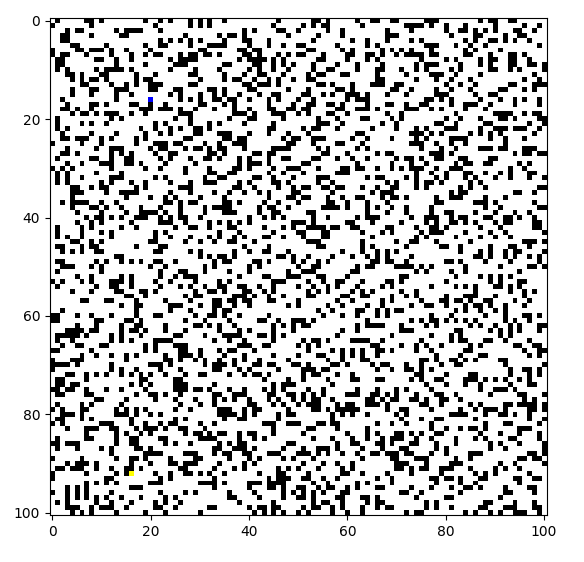
\includegraphics[width=0.75\textwidth]{fig1.png}
    \caption{Maze000 Initial Conditions}
    \label{fig:Maze000}
\end{figure}

Our solution contains a method called showInitialMaze which takes in a file of the format of problem.txt and builds a maze object and visualizes the maze with the start and end points and black boxes as the barriers. An example of maze000.txt with a start point of (16, 20) and a goal of (92, 16) is shown below where blue is the start point and yellow is the goal point. 
\newpage

\section*{{Analysis}}
\textit{1. Algorithm 0: Uniform Cost Search}
\begin{itemize}
    \item Completeness: UCS is considered complete, as it will consider all paths systematically, in order of increasing cost, never getting caught going down a single infinite path.
    \item Optimal: UCS is optimal as the first solution it finds will have a cost at least as low as the cost of any other node in the frontier.
    \item Comparison to Breadth-First Search: Similar to UCS, BFS is considered complete as it will generate all possible paths, thus if one of these paths are a solution, it will be found. However, it is only cost optimal when every action costs the same. Thus, BFS will not be optimal for our problem.
\end{itemize}
Running the UCS algorithm on the initial problem described in the setup above, the following path is found. It has a cost of 176 and took .0217 seconds to compute. The red cells are all the visited cells and the green shows the path from start state to the goal state.
\begin{figure}[ht]
    \centering
    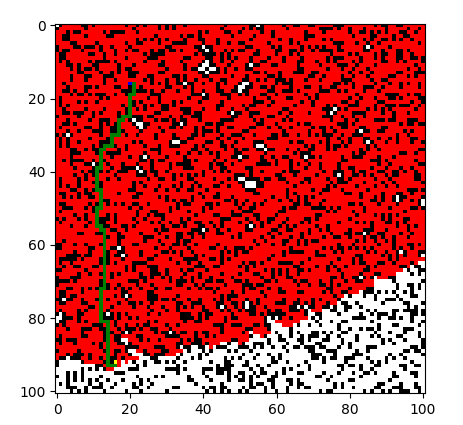
\includegraphics[width=0.75\textwidth]{fig2.png}
    \caption{Uniform Cost Search on Initial Problem}
    \label{fig:UCS}
\end{figure}
\newline
Looking at the area the algorithm searches, it actually covers a relatively large amount of the maze before finding the optimal path. This is due to the min heap that is used to sort by cost, meaning that nodes that are far away from the goal will still be considered if their cost is low enough. Compared to some algorithms that consider heuristics such as A*, this could become inefficient as the size of the maze and the distance between the start and goal stats becomes very large.

\newpage

\textit{2. Algorithm 1: Iterative Deepening Depth-First Search}
\begin{itemize}
    \item Completeness: IDDFS is considered complete since our problem is a finite space and returns a solution if one exists.
    \item Optimal: IDDFS is not optimal for this problem since the cost of some actions are different.
\end{itemize}
Running the IDDFS algorithm on the initial problem described in the setup above, the following path is found. It has a cost of 784 and took 2.577 seconds to compute. The red cells are all the visited cells and the green shows the path from start state to the goal state.

\begin{figure}[ht]
    \centering
    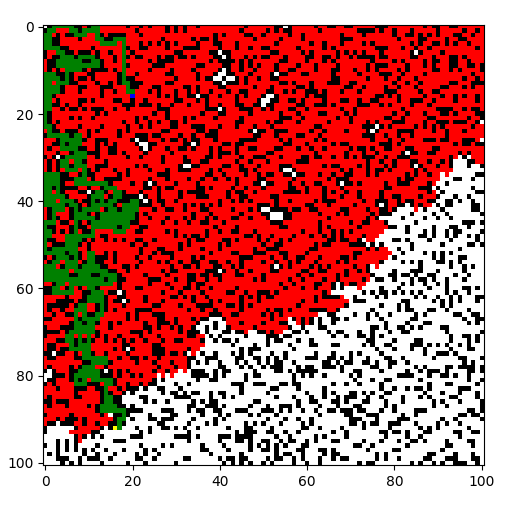
\includegraphics[width=0.75\textwidth]{fig3.png}
    \caption{Iterative Deepening Depth-First Search on Initial Problem}
    \label{fig:IDDFS}
\end{figure}

Comparing the searched area from IDDFS to UCS, it appears that IDDFS searches less of the maze despite taking far more time than UCS. This is because it iterates through the Depth Limited Search algorithm, incrementing the max depth by 1 each time the search fails untils it hits a maximum allowable depth. Because of this it is actually running the Depth Limited Search for many iterations before finding a solution. Another issue is that the DLS algorithm does not find an optimal solution as the path is randomly determined by the specific order in which DLS searches its neighbors. Thus, the path is often much more complicated than it should be, however the path does not form cycles or overlap itself. The cost found for this algorithm is extremely high at 784, showing that this algorithm is probably not the best one to choose. Perhaps it could be useful if the max travelable distance was known before solving the problem, thus the algorithm would terminate after it could not find a solution that satisfies the cost constraint while other algorithms would continue searching.

\newpage

\textit{3. Algorithm 2: A* with Manhattan distance $(h_1)$}
\begin{itemize}
    \item Consistent: For our problem, A* Using Manhattan distance is considered consistent, as the first time we reach a new state, we are guaranteed to be on an optimal path. Thus, the function h(n) never becomes greater than the cost of the action from n to n’ plus the heuristic estimate.
    \item Admissible: Assume h1 is admissible. Let $n$ be a node such that the goal function $g(n)$ is valid but is part of a non optimal path. Let $n’$ be a node on the optimal path. Observing that the Manhattan distance is very similar to the triangle inequality which states that the sum of two sides of a triangle is always greater than or equal to the third side, it becomes clear that the Manhattan distance is actually the minimum cost of getting to the goal state. This is because the Manhattan distance will always be greater than or equal to the actual cost of getting to a goal state given the movement restrictions, the actual cost of getting the goal state will always be along the Manhattan distance due to the movement restrictions. In this problem the following equality will hold where c* is the cost of moving the non optimal node to the goal state:

$f(n’) = g(n’) + h(n’) <= c* < f(n) = g(n) + h(n)$

Thus, A* with h1 will always expand the n’ node with the lower cost function and will never overestimate and is therefore admissible

\end{itemize}
Running the A* algorithm with Manhattan distance as the heuristic on the initial problem described in the setup above, the following path is found. It has a cost of 176 and took .0154 seconds to compute. The red cells are all the visited cells and the green shows the path from start state to the goal state.

\begin{figure}[ht]
    \centering
    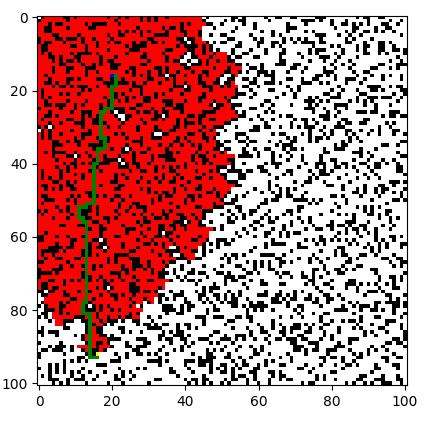
\includegraphics[width=0.75\textwidth]{fig4.png}
    \caption{A* using Manhattan Distance on Initial Problem}
    \label{fig:h1}
\end{figure}
The A* algorithm with manhattan distance as the heuristic significantly reduces the searched part of maze as shown in Figure 4 compared the other previous algorithms. It has the fastest time to compute at only .0154 seconds and results in the same optimal cost as UCS. This algorithm would likely scale much better than UCS to more complex and larger mazes, as the search area from UCS scales very fast as the complexity of the problem increases. It seems that Manhattan distance is an excellent heuristic for solving maze problems.
\newpage

\textit{4. Algorithm 3: A* with Minimum of Euclidean and Manhattan $(h_3)$}
\begin{itemize}
    \item Consistent: This algorithm uses either the euclidean distance or Manhattan distance to a goal state, whichever one is smaller due to the minimum function. Thus, as long as both the  Euclidean distance and Manhattan distance are consistent, this heuristic will also be consistent as it will always be less than or equal to two proven consistent heuristics.  We have already shown that Manhattan distance is consistent. Euclidean distance is also consistent by a very similar proof. Considering the fact that Euclidean distance is the shortest distance possible from two points assuming no obstructions, then it is clear that the Euclidean distance will always be less than or equal to the Manhattan distance (which can also be seen from the triangle inequality). Thus it is clear that the Euclidean distance is consistent, and thus the minimum of these two heuristics is also consistent.
    \item Admissible: The Manhattan distance heuristic has already been shown to be admissible. Euclidean distance heuristic is also known to be admissible as it calculates a direct path to the goal, ignoring any barricades or even invalid paths and actions. As such, the cost of the current state to the goal will never be overestimated and thus this heuristic is consistent.
\end{itemize}
Running the A* algorithm with the minimum of the Manhattan and euclidean distance as the heuristic on the initial problem described in the setup above, the following path is found. It has a cost of 176 and took .0218 seconds to compute. The red cells are all the visited cells and the green shows the path from start state to the goal state.

\begin{figure}[ht]
    \centering
    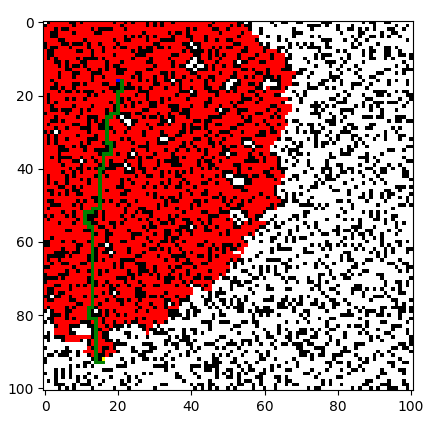
\includegraphics[width=0.75\textwidth]{fig5.png}
    \caption{A* using Minimum of Euclidean and Manhattan Distance on Initial Problem}
    \label{fig:h3}
\end{figure}
The A* algorithm with the minimum of the Manhattan and Euclidean distance as the heuristic has a searched area in between that of UCS and Algorithm 2. While this may seem like it is slightly worse than using just the Manhattan distance, having a slightly larger search area could be beneficial if the maze has many dead ends and other obstacles as the algorithm could develop more paths to circumvent these obstructions. For this particular maze its time is slightly slower than algorithm 2 at .0218 seconds, however more iterations of all the algorithms will be compared in the next section.
\newpage
\textit{5. Algorithm 4: A* with custom heuristic}
\begin{itemize}
    \item $h_6 = min{w*h1(n) (1-w), w*h2(n) (1-w)}, w = rand(0, 1), h_1 = Manhattan, h_2 = Euclidean$
    \item Consistent: It is very easy to see that heuristic will always be less than or equal to the previously discussed $h_3$ due to the added probability which only scales the value between (0, 1). Thus because $h_3$ is consistent, so is this custom heuristic.

    \item Admissible: The heuristic takes the minimum of a randomly (between 0.0 and 1.0) scaled Manhattan and Euclidean distance heuristic. As such, the heuristic is only ever as big as either its Manhattan or Euclidean counterpart. With this being the case, the estimated costs will always be smaller than the actual costs. Thus, the custom heuristic is admissible.
    \item Better than others?: This question will be explored after examining the data found in the next section.
\end{itemize}
Running the A* algorithm with the custom heuristic on the initial problem described in the setup above, the following path is found. It has a cost of 176 and took .0335 seconds to compute. The red cells are all the visited cells and the green shows the path from start state to the goal state.


\begin{figure}[ht]
    \centering
    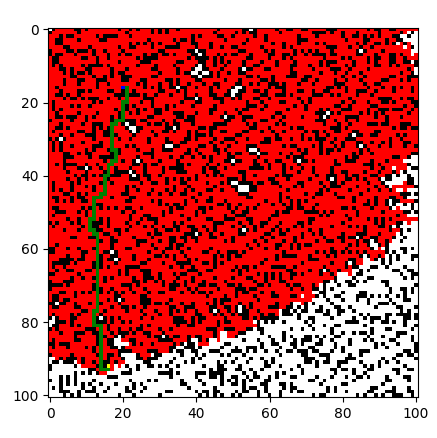
\includegraphics[width=0.75\textwidth]{fig6.png}
    \caption{A* using Custom Heuristic on Initial Problem}
    \label{fig:custom}
\end{figure}
The A* algorithm with the custom heuristic has a searched area that is larger than the previous A* implementations. Having a slightly larger search area that involves essentially searching over a wider probability distribution could be beneficial if the maze has many dead ends and other obstacles as the algorithm could develop more paths to circumvent these obstructions. For this particular maze its time is slightly slower than algorithm 2 at .0335 seconds, which is directly due to the increased cost of computing the heuristic and the expanded search area. More discussion on why the heuristic was chosen and how it compares will be done in the next section. 
\newpage

\section*{{Results}}
\textit{In this section each algorithm was tested 50 times from maze000 to maze049. The start and goal points were randomized to valid initial positions and were kept consistent through each iteration. The time taken to complete each algorithm as well as the reported cost of a solution were both recorded over the run. A cost of zero is associated with a failed search. The goal of this section is to analyze the performance and behavior of each algorithm.}

\begin{figure}[ht]
    \centering
    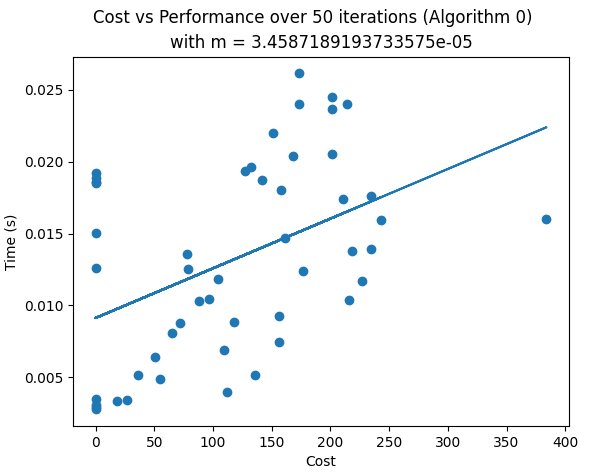
\includegraphics[width=\textwidth]{CVPALG0.png}
    \caption{Cost vs Performance over 50 iterations using Uniform Cost Search}
    \label{fig:CostVsPerformanceAlg0}
\end{figure}
\newpage
\begin{figure}[ht]
    \centering
    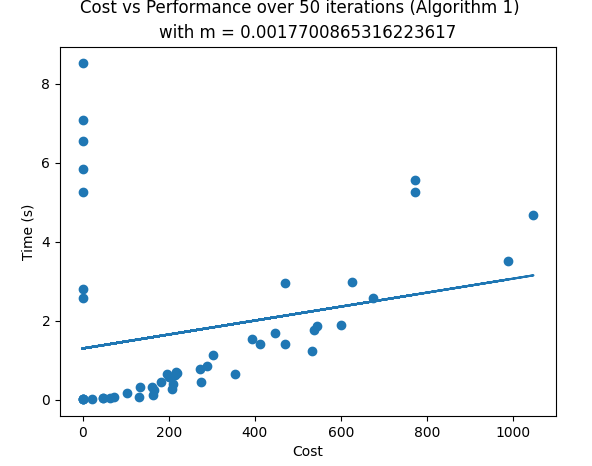
\includegraphics[width=\textwidth]{CVPALG1.png}
    \caption{Cost vs Performance using Iterative Deepening Depth First Search}
    \label{fig:CostVsPerformanceAlg1}
\end{figure}
Comparing the first two algorithms shown in Figure 7 and 8, it becomes clear that IDDFS is significantly slower and overall worse performing than the UCS algorithm. Not only does it typically achieve much higher cost solutions, it takes orders of magnitude more time to compute these solutions. As a worse case when no solution is found, it could take up to 8 seconds to compute that there is no path where the highest time taken by UCS is only .025 seconds. This performance discrepancy is so big that there are almost no use cases where IDDFS would be recommended. While neither of these plots are particularly linear, a simple linear regression does give some interesting intuition on how these algorithms might scale given a more complex maze. The slope represents how the cost of a solution dictates the time found to a solution. Meaning that a maze with a very long path will generally take a longer time to solve than one with a smaller optimal path. As seen by the regression, the UCS has a much smaller slope than IDDFS, indicating that as maze complexity increases the gap between the time taken to find a solution will grow wider as well (assuming a suitable depth for IDDFS). It should be noted that given more data over larger maze sizes, a better fit could be adapted to show the accurate growth of these algorithms.
\newpage
\begin{figure}[ht]
    \centering
    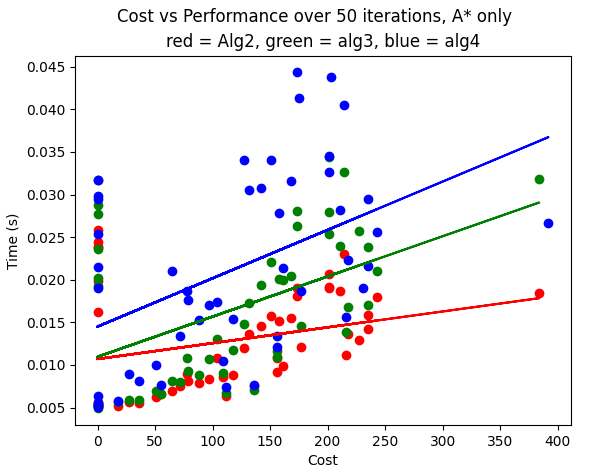
\includegraphics[width=\textwidth]{AstarCompare.png}
    \caption{ Cost vs Performance over 50 iterations using A* search, all heuristics plotted}
    \label{fig:CostVsPerformanceAstar}
\end{figure}
In figure 9, we compare the cost vs performance between each A* search implemented with different heuristics. From this, we see that the heuristics chosen had a significant impact on performance. Interestingly, algorithm three and four exhibit similar rates of growth, indicating that as the maze size gets very large the performance of these algorithms will likely approach the same value. From the data it is clear that algorithm four generally takes the most time to compute a solution and algorithm 2 takes the least amount of time to find a solution. Overall, UCS and algorithm 2 appear to be the best algorithms while IDDFS is clearly the worst performing.  
\newpage
\begin{figure}[ht]
    \centering
    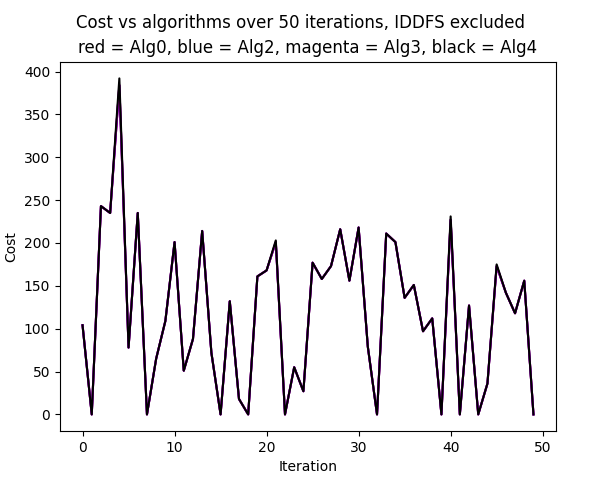
\includegraphics[width=\textwidth]{CVA50N.png}
    \caption{Cost vs Algorithm, Iterative Deepening Depth First Search excluded}
    \label{fig:CostVsAlgs}
\end{figure}
For this graph, we intentionally excluded IDDFS. The reason for this is due to how much of an outlier data from IDDFS produces. In any case, from this graph, we see that despite using different heuristics, all of the A* search algorithms performed with the same cost. Additionally, using Uniform Cost Search, an uninformed search algorithm, also shared the same cost as A*. From this, we gather not only that UCS is as cost optimal compared to an informed search algorithm, but that it is also as consistent as well. From this graph it is clear that not only are all the algorithms optimal, they are also consistent amongst themselves.
\newpage
\begin{figure}[ht]
    \centering
    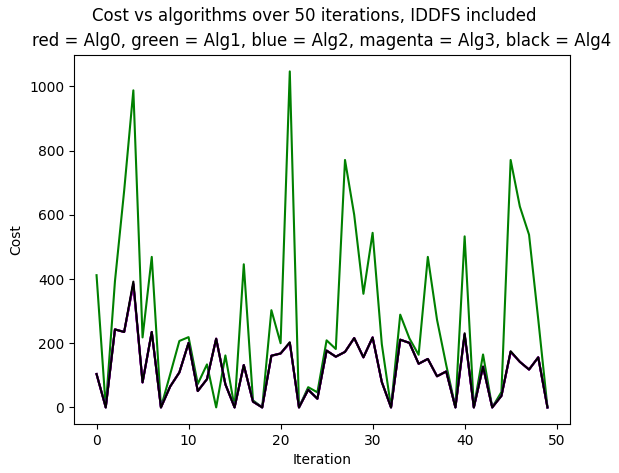
\includegraphics[width=\textwidth]{CVA50IDDFS.png}
    \caption{Cost vs Algorithms, including Iterative Deepening Depth First Search}
    \label{fig:CostVsAlgsIDDFS}
\end{figure}
For completeness, we have included IDDFS this time. As shown, IDDFS far exceeds the cost used compared to other algorithms implemented. Compared to other algorithms, IDDFS takes far longer, and costs much more despite searching less cells. In addition the results where IDDFS has a value of zero is when it can not find a solution. The two figures shown below indicate the average performance of the algorithms over the 50 iterations (excluding IDDFS because of scaling issues).

\newpage
\begin{figure}[ht]
    \centering
    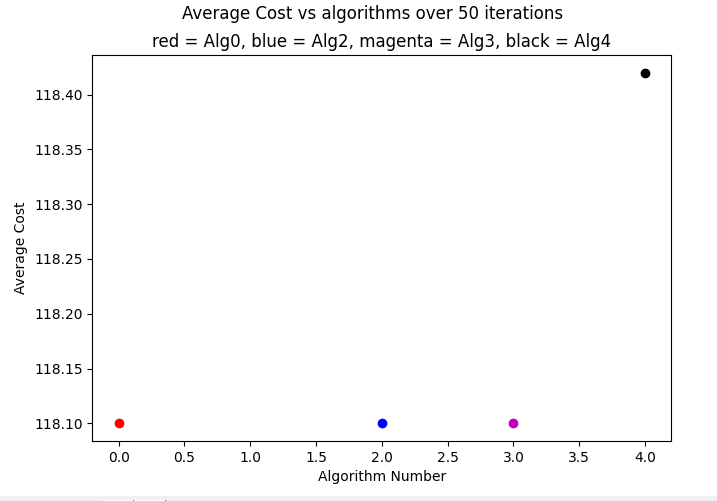
\includegraphics[width=\textwidth]{avgcost.png}
    \caption{Average Cost of Algorithms, excluding Iterative Deepening Depth First Search}
    \label{fig:avgcost}
\end{figure}
\newpage
\begin{figure}[ht]
    \centering
    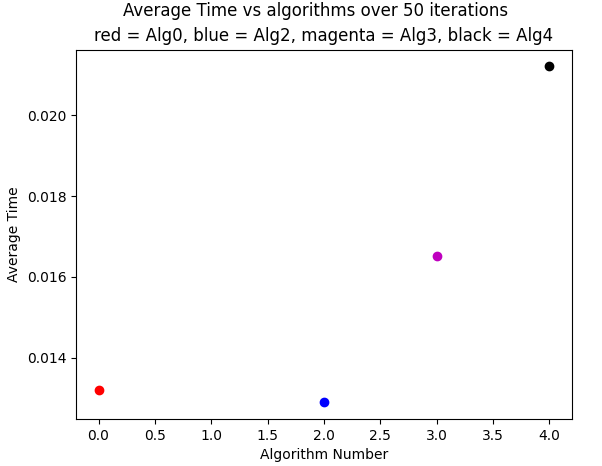
\includegraphics[width=\textwidth]{avgtime.png}
    \caption{Average Time of Algorithms, excluding Iterative Deepening Depth First Search}
    \label{fig:avgtime}
\end{figure}
As shown in Figure 12, the average cost of all the algorithms is extremely close at nearly all having the same average cost (the custom heuristic interestingly is slightly higher but overall it is a very marginable difference). Figure 13 gives some very interesting information regarding how the algorithms perform relative to each other. It appears that Algorithm 2 which uses the Manhattan distance as the heuristic is the best performing algorithm with UCS very close by. Algorithm 3 is then slightly worse performing, with the algorithm 4 and the custom heuristic performing the worst. Despite this, it is still very difficult to decide what heuristic is the ‘best’ due to the relatively small sample size and lack of scaling of maze size and complexity. To further test these algorithms larger mazes with more deadends between the start and goal state would likely show the advantages of heuristics that investigate more of the maze and may even result in these algorithms outperforming UCS and Algorithm 2.
\par
The decision to design the custom heuristic as h6 = min{w*h1(n) (1-w), w*h2(n) (1-w)}, w = rand(0, 1), h1 = Manhattan, h2 = Euclidian, was to allow for more of the maze to be searched. The thought process was that more stochasity would give the algorithm a better performance in solving really complicated mazes while still keeping the benefits of an informed search algorithm. While for very simple cases where the optimal path is very close to say the Euclidean path the custom heuristics will be outperformed as it searches more nodes, it may find a solution earlier given many obstructions and a large maze. Comparing the informed searches vs UCS would display an interesting result as the size of the maze gets very large and the optimal path becomes long. Because UCS is uninformed, it will grow its frontier out in a circular-like pattern, searching nodes which could be getting further away from the actual goal point without knowing. Thus UCS will take very long to find paths that start in the center of a large maze compared to the informed searches. Overall the performance of the custom heuristic is still unclear, but in general on small mazes that don’t have many obstruction A* with manhattan distance will likely be the best algorithm, but as the complexity and size of the maze increase more research would need to be done to determine which algorithm to select. A major outcome is to avoid using IDDFS due it being non optimal and a very slow algorithm compared to all the other tested algorithms.

\end{document}